% Claim2Value · 复赛展示稿
% 编译：latexmk -xelatex -interaction=nonstopmode slides.tex
\documentclass[aspectratio=169,11pt]{ctexbeamer}

\usetheme{metropolis}

\usepackage{fontspec}
\usepackage{booktabs,array,tabularx,amsmath,amssymb}
\usepackage{tikz}
\usetikzlibrary{arrows.meta,positioning}
\usepackage{pgfplots}
\pgfplotsset{compat=1.18}
\usepackage{graphicx}

% ---------- 品牌色 ----------
\definecolor{ink}{HTML}{25272B}
\definecolor{muted}{HTML}{62666B}
\definecolor{linec}{HTML}{DEDEDB}
\definecolor{accentc}{HTML}{763B32}
\definecolor{accentsoftc}{HTML}{C49D95}
\definecolor{trackc}{HTML}{E8E6E2}
\definecolor{softbgc}{HTML}{F7F6F4}

\setbeamercolor{normal text}{fg=ink,bg=white}
\setbeamercolor{frametitle}{fg=ink,bg=white}
\setbeamercolor{structure}{fg=accentc}
\setbeamercolor{alerted text}{fg=accentc}
\setbeamercolor{title}{fg=ink}
\setbeamercolor{subtitle}{fg=accentc}
\setbeamercolor{author}{fg=muted}
\setbeamercolor{progress bar}{fg=accentc,bg=trackc}
\setbeamercolor{title separator}{fg=accentc}
\setbeamercolor{block title}{fg=white,bg=accentc}
\setbeamercolor{block body}{fg=ink,bg=softbgc}

\setbeamerfont{title}{size=\Huge,series=\bfseries}
\setbeamerfont{subtitle}{size=\large}
\setbeamerfont{frametitle}{size=\Large,series=\bfseries}
\setbeamerfont{block title}{size=\small,series=\bfseries}

\metroset{block=fill,numbering=fraction,progressbar=frametitle,sectionpage=progressbar}

% ---------- 中文字体（可变字体按文件调用） ----------
\setsansfont{Fira Sans}
\setCJKsansfont{NotoSansSC-VF.ttf}[Path=C:/Windows/fonts/,BoldFont=NotoSansSC-VF.ttf,AutoFakeBold=1.6]
\setCJKmainfont{NotoSansSC-VF.ttf}[Path=C:/Windows/fonts/,BoldFont=NotoSansSC-VF.ttf,AutoFakeBold=1.6]
\renewcommand{\familydefault}{\sfdefault}

\newcommand{\kw}[1]{\textcolor{accentc}{\bfseries #1}}
\newcommand{\code}[1]{{\ttfamily\small\detokenize{#1}}}

\setbeamertemplate{footline}{%
  \hfill{\usebeamerfont{footline}\color{muted}\small
  Claim2Value · 饮水思源 · 2026-10-12\hspace{1em}}\vskip4pt}

\title{Claim2Value}
\subtitle{面向机器人产业链的财务研究工作台}
\author{饮水思源}
\institute{北京大学金融 AI 智能体创新大赛 · 复赛}
\date{2026 年 10 月 12 日}

\begin{document}

\begin{frame}[plain]
\titlepage
\end{frame}

\begin{frame}{团队与分工}
\vspace{0.2cm}
\begin{tabularx}{\textwidth}{@{}l l X@{}}
\toprule
\bfseries 姓名 & \bfseries 单位 & \bfseries 分工 \\
\midrule
魏孟祺 & 西安交通大学 · 金禾经济研究中心 & 负责人。项目构建、需求判断与规划 \\
孙圣尧 & 上海交通大学 · 巴黎卓越工程师学院 & 项目测试、资料搜集与前端优化 \\
陈洛笛 & 西安交通大学 · 计算机学院 & 代码实现、测试与 review \\
\bottomrule
\end{tabularx}

\vspace{0.6cm}
\begin{block}{本次展示}
一个本地部署的财务研究工作台。验证案例：绿的谐波（688017）2024 年年度报告，13 页，公开披露原件。
\end{block}
\end{frame}

\begin{frame}{问题：数字脱离了它成立的条件}
\vspace{0.1cm}
\begin{columns}[T,onlytextwidth]
\begin{column}{0.31\textwidth}
\begin{block}{技术表述}
「减重 30\%」不说同等输出扭矩、不说比较对象、不说统计口径，就无法复核。
\end{block}
\end{column}
\begin{column}{0.31\textwidth}
\begin{block}{报表范围}
合并报表与母公司报表并列排版，同一指标两处数值不同。利润总额、所得税、净利润最容易错配。
\end{block}
\end{column}
\begin{column}{0.31\textwidth}
\begin{block}{单位与期间}
「台」与「万台」相差 $10^4$；年度累计与单季、原版与更正只差一两个字。
\end{block}
\end{column}
\end{columns}

\vspace{0.4cm}
\begin{alertblock}{这类错误的特点}
看起来完全正常。人工复制粘贴时很难自查，因为它不违反任何直观印象。
\end{alertblock}
\end{frame}

\begin{frame}{方案：先固定证据，再作判断}
\vspace{0.5cm}
\begin{center}
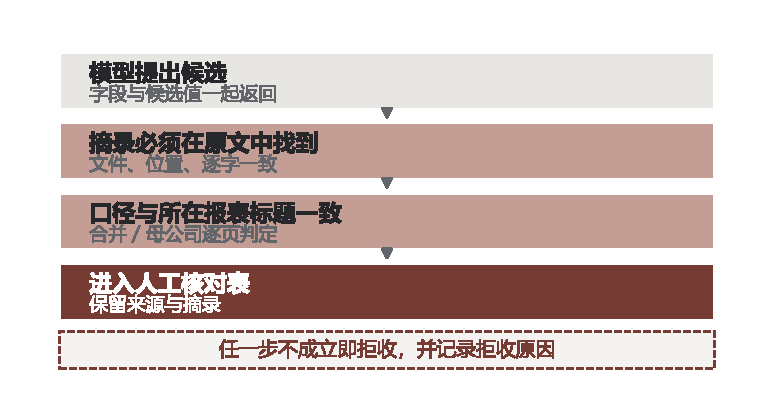
\includegraphics[width=0.9\textwidth]{figures/fig_mechanism.pdf}
\end{center}
\vspace{0.2cm}
\begin{itemize}
  \item 每条候选必须携带\kw{逐字原文摘录}，并指回具体文件与页码。
  \item 通过摘录检查后，再核对声明的报表范围与所在页标题是否一致。
  \item 任一步不成立即拒收，拒收原因留存，不进入下载包。
\end{itemize}
\end{frame}

\begin{frame}{架构与边界}
\vspace{0.3cm}
\begin{center}
\begin{tikzpicture}[
  font=\sffamily\small, node distance=5mm,
  box/.style={draw=linec,fill=white,rounded corners=1.2mm,minimum height=8mm,inner xsep=6pt,align=center,text=ink},
  rule/.style={draw=accentc,fill=softbgc,rounded corners=1.2mm,minimum height=8mm,inner xsep=6pt,align=center,text=ink},
  svc/.style={draw=linec,fill=trackc,rounded corners=1.2mm,minimum height=7mm,inner xsep=6pt,align=center,text=muted},
  ->,>=Stealth,thick,draw=muted]
\node[box,minimum width=24mm] (a) {原件};
\node[box,right=9mm of a,minimum width=26mm] (b) {解析与分片};
\node[rule,right=9mm of b,minimum width=34mm] (c) {本机规则};
\node[box,right=9mm of c,minimum width=26mm] (d) {人工核对表};
\draw (a)--(b); \draw (b)--(c); \draw (c)--(d);
\node[svc,below=6mm of b,minimum width=26mm] (m) {自备模型接口};
\draw[dashed] (b)--(m);
\node[svc,below=6mm of c,minimum width=34mm] (l) {本地计算};
\draw[dashed] (c)--(l);
\end{tikzpicture}
\end{center}

\vspace{0.2cm}
\begin{columns}[T,onlytextwidth]
\begin{column}{0.48\textwidth}
\begin{block}{自研}
证据规则与口径检查、记录与留痕、工程到财务的映射、回测时序、界面与交互。
\end{block}
\end{column}
\begin{column}{0.48\textwidth}
\begin{block}{外部}
自备大模型接口（可完全不用）；Streamlit / pandas / NumPy / PyArrow / pypdf。
\end{block}
\end{column}
\end{columns}

\vspace{0.15cm}
本机规则部分\kw{不调用任何模型}：核验、数据体检、盈利变化、回测全部本地完成，无需密钥。
\end{frame}

\begin{frame}{机制一：引用锚定}
\vspace{0.4cm}
每条候选必须存在原文片段 $p$，使下式同时成立：

\vspace{0.35cm}
\begin{center}
\code{quote} $\subset$ \code{text}(p), \quad
\code{p.source\_file} $=$ \code{source\_file}, \quad
\code{p.source\_locator} $=$ \code{source\_locator}
\end{center}

\vspace{0.45cm}
\begin{alertblock}{这条规则改变了什么}
把「模型说某个数字是 6,076 万」——无法核对——变成「模型说第 112 页出现了这句话」——可以立刻核对。不成立的候选写入拒收清单，附序号与声称的字段值。
\end{alertblock}
\end{frame}

\begin{frame}{机制二：报表口径校验}
\vspace{0.25cm}
标题用严格的整行匹配，正文里提到这些字样不算标题：

\vspace{0.25cm}
\code{(合并|母公司)(资产负债表|利润表|现金流量表|所有者权益变动表)}

\vspace{0.4cm}
\begin{itemize}
  \item 按页码顺序做\kw{跨页继承}：页首无新标题且页码连续时，沿用上一页最后一个生效标题。
  \item 校验时取出该摘录在整页中的\kw{每一次}出现，各自定位到当时生效的标题。
  \item 只有所有出现处口径一致、且与声明冲突时才拒收；标题不明则\kw{不作判断}。
\end{itemize}

\vspace{0.3cm}
\begin{block}{为什么需要这一步}
模型按页看文本，看不到「这一页属于哪张报表」；标题印在上一页页末时，单页成批就丢了上下文。
\end{block}
\end{frame}

\begin{frame}{机制三与四：单位相邻、回测时序}
\vspace{0.3cm}
\begin{columns}[T,onlytextwidth]
\begin{column}{0.47\textwidth}
\begin{block}{单位相邻校验}
数值与单位必须在原文中明确相连，用带前置断言的正则检查。不满足即拒收，避免把「台」误读成「万台」。
\end{block}
\end{column}
\begin{column}{0.47\textwidth}
\begin{block}{回测时序}
T 日收盘后形成信号，T+1 日收盘成交，T+2 日开始计入收益。因子须给出带时分时区的可得时间，超过当日 15:00 不参与当日信号。
\end{block}
\end{column}
\end{columns}

\vspace{0.5cm}
\begin{center}

\includegraphics[width=0.86\textwidth]{figures/fig_timing.pdf}
\end{center}
\end{frame}

\begin{frame}{与常见做法的对照}
\vspace{0.2cm}
\begin{tabularx}{\textwidth}{@{}p{0.32\textwidth}X@{}}
\toprule
\bfseries 常见做法 & \bfseries 本项目 \\
\midrule
整份年报交给模型直接要结论 & 按页与片段切分，每条候选必须能指回具体片段 \\
模型给出的数字直接采信 & 数值必须伴随可在原文中找到的逐字摘录 \\
合并与母公司混用，事后人工检查 & 按页识别标题并跨页继承，生成阶段即拦截 \\
只输出最终报告 & 同时输出拒收清单与原因，失败批次留为缺口，可断点继续 \\
\bottomrule
\end{tabularx}
\end{frame}

\section{效果与效率}

\begin{frame}{同一份原件的两轮对比}
\vspace{0.1cm}
\begin{center}
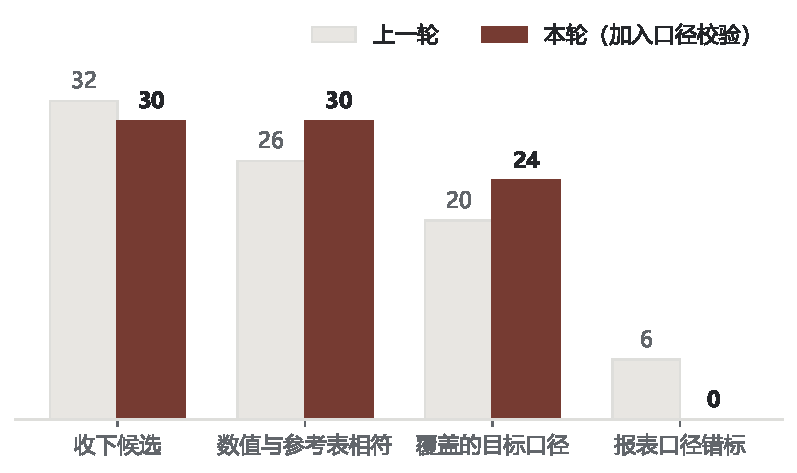
\includegraphics[width=0.86\textwidth]{figures/fig_two_round.pdf}
\end{center}
\vspace{0.05cm}
第二轮加入口径校验：候选数略降，与参照表相符的条数与覆盖的目标口径同时上升，口径错标归零。
\end{frame}

\begin{frame}{24 个目标口径的覆盖}
\vspace{0.1cm}
\begin{center}
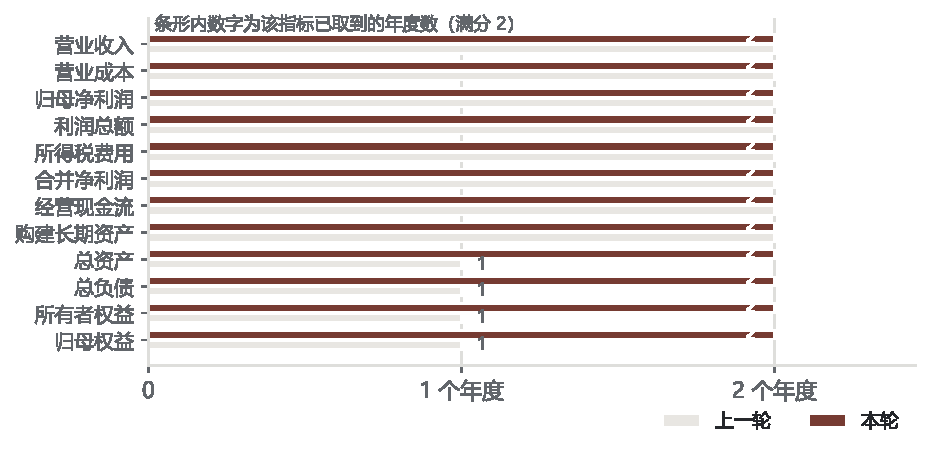
\includegraphics[width=0.8\textwidth]{figures/fig_coverage.pdf}
\end{center}
\vspace{0.05cm}
上一轮在资产、负债、所有者权益与归母权益四项上只取到一个年度；第二轮全部取满两个年度。
\end{frame}

\begin{frame}{案例：被错标的 6 条}
\vspace{0.15cm}
\begin{columns}[T,onlytextwidth]
\begin{column}{0.56\textwidth}
\small
\begin{tabular}{@{}l r r@{}}
\toprule
\bfseries 指标 & \bfseries 错取值 & \bfseries 参照值 \\
\midrule
利润总额（2024） & 64,572,784.68 & 60,764,068.46 \\
利润总额（2023） & 91,985,161.50 & 91,571,396.66 \\
所得税（2024） & 5,525,057.09 & 4,955,333.81 \\
所得税（2023） & 9,176,871.02 & 6,739,185.62 \\
净利润（2024） & 59,047,727.59 & 55,808,734.65 \\
净利润（2023） & 82,808,290.48 & 84,832,211.04 \\
\bottomrule
\end{tabular}

\vspace{0.15cm}
{\footnotesize 单位：元。错取值取自第 114 页母公司利润表，参照值取自第 112 页合并利润表。}
\end{column}
\begin{column}{0.41\textwidth}
\begin{block}{成因}
第 114 页\kw{自身没有报表标题}——「母公司利润表」印在第 113 页页末。单页成批后标题丢失，模型误以为延续第 112 页的合并利润表。
\end{block}

\begin{block}{隔离验证}
离线复放第一轮的 32 条候选（不调用模型）：恰好标出第 23--28 号这 6 条，未误伤其余 26 条，漏标 0 条。
\end{block}
\end{column}
\end{columns}
\end{frame}

\begin{frame}{盈利变化分解（真实数据）}
\vspace{0.05cm}
\begin{center}
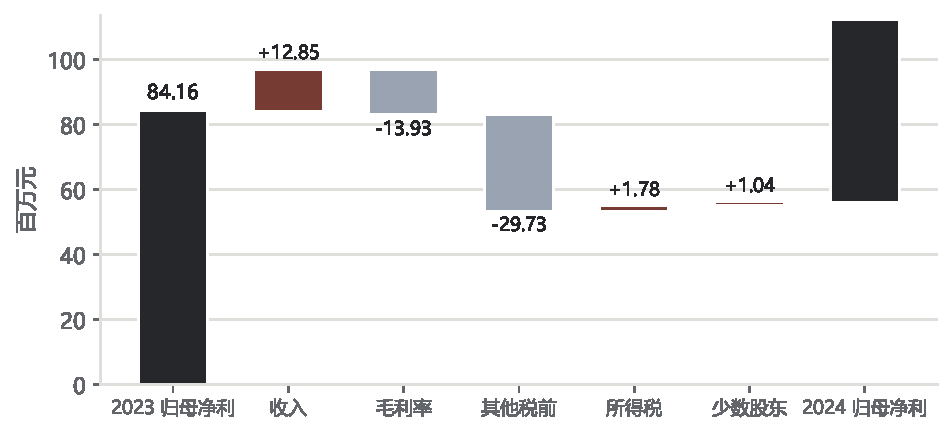
\includegraphics[width=0.78\textwidth]{figures/fig_bridge.pdf}
\end{center}
\vspace{-0.05cm}
{\small 收入增长带来的 $+1{,}285$ 万元贡献，被毛利率从 41.14\% 降到 37.54\% 造成的 $-1{,}393$ 万元抵消并超过；其余税前项目净减 $2{,}973$ 万元。}
\end{frame}

\begin{frame}{效率与成本}
\vspace{0.1cm}
\begin{center}
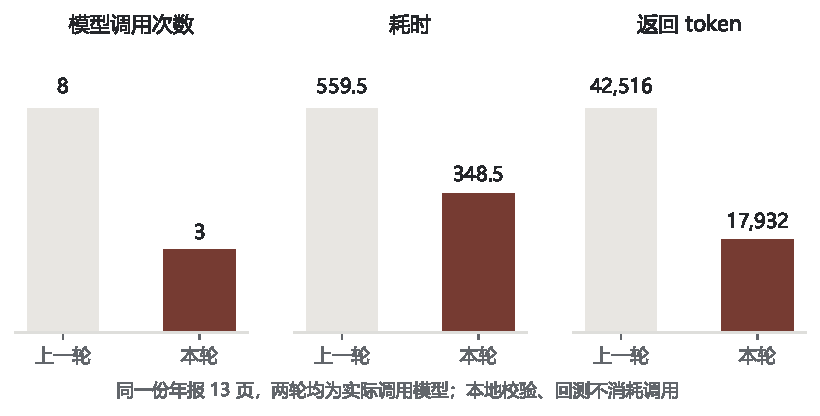
\includegraphics[width=0.88\textwidth]{figures/fig_efficiency.pdf}
\end{center}
\vspace{0.1cm}
\begin{columns}[T,onlytextwidth]
\begin{column}{0.48\textwidth}
\begin{block}{两轮实测}
调用 8 次 → 3 次；耗时 559.5 秒 → 348.5 秒；返回 token 42,516 → 17,932。
\end{block}
\end{column}
\begin{column}{0.48\textwidth}
\begin{block}{本地部分}
核验、数据体检、盈利变化与回测\kw{调用 0 次}，不产生模型费用。工作台自带 557 项测试全部通过。
\end{block}
\end{column}
\end{columns}
\end{frame}

\section{适用性与呈现}

\begin{frame}{怎么用}
\vspace{0.2cm}
\begin{tabularx}{\textwidth}{@{}lX@{}}
\toprule
\bfseries 项目 & \bfseries 说明 \\
\midrule
启动 & 双击 \code{start\_harness.bat}（Windows）或 \code{bash start\_harness.sh} \\
访问 & 浏览器打开 \code{http://127.0.0.1:8510}，无需账号 \\
环境 & Python 3.12，首次安装依赖需联网 \\
密钥 & 本地计算不需密钥；仅提取与检索需自备模型接口 \\
\bottomrule
\end{tabularx}

\vspace{0.45cm}
\begin{block}{典型路径}
上传年报并选择页码 → 提取候选或导入已整理长表 → 对照原件核对 16 个字段 → 校验 → 生成成果、盈利变化与可选 DCF。
\end{block}
\end{frame}

\begin{frame}{稳定性与需要人工确认的环节}
\vspace{0.2cm}
\begin{columns}[T,onlytextwidth]
\begin{column}{0.48\textwidth}
\begin{block}{异常处理}
失败批次留为缺口，其余继续；再次点击只请求未完成部分。上下文超限按片段拆小重试，最多四层。网络中断有限重试，认证与额度问题立即停止。
\end{block}
\end{column}
\begin{column}{0.48\textwidth}
\begin{block}{必须由人确认}
字段映射是否正确；数据缺口是否接受（缺披露日 14 条、缺修订标记 30 条、缺代码 16 条、6 组重复）；估值参数是否为使用者自己的假设。
\end{block}
\end{column}
\end{columns}

\vspace{0.4cm}
\begin{alertblock}{边界}
扫描件需先自行 OCR；无可识别标题的页面不作口径判断；回测未模拟停牌、涨跌停、冲击成本；已查看过的区间不构成未触碰留出集。Windows 11 已验收，Linux 未真机验证。
\end{alertblock}
\end{frame}

\begin{frame}{初赛后的深化}
\vspace{0.15cm}
\small
\begin{tabularx}{\textwidth}{@{}p{0.18\textwidth}X X@{}}
\toprule
\bfseries 方面 & \bfseries 初赛 & \bfseries 本次 \\
\midrule
产品形态 & 固定案例演示程序 & 可上传自备文件的研究工作台，本地部署可启动 \\
财务提取 & 模型返回字段，人工核对 & 加入引用锚定与口径校验，展示未采用候选与原因 \\
验证方式 & 单轮人工抽查 & 两轮实测对照 + 离线复放隔离验证，24 个口径逐条比对 \\
数据体检 & 无 & 回测前检查列映射、代码、日期、重复、缺失与因子可得时间 \\
运行记录 & 过程不落盘 & 运行目录留原件、中间状态与拒收原因，支持断点续取 \\
\bottomrule
\end{tabularx}
\end{frame}

\begin{frame}{下一步与结语}
\vspace{0.3cm}
\begin{block}{下一步}
扩展案例到不同行业与披露格式，识别规则失效边界；把单位与口径校验覆盖到全部财务指标；补齐数据库字段的正式定义；在产品内做逐条件进度提示。
\end{block}

\vspace{0.5cm}
\begin{center}
{\Large\bfseries\color{accentc} 先固定证据，再作判断。}

\vspace{0.35cm}
{\large 饮水思源\enspace·\enspace Claim2Value}

\vspace{0.25cm}
{\small\color{muted} 全部收据见 05\_技术证据/，逐条可核对}
\end{center}
\end{frame}

\end{document}
